\documentclass[12pt,a4paper]{report}
					
					\usepackage[titles]{tocloft}
					\newlength{\mylen} % a scratch length
					\renewcommand{\cftfigpresnum}{Gambar } % goes before figure number
					\settowidth{\mylen}{\cftfigpresnum} % space required to print \cftfigpresnum
					\addtolength{\mylen}{\cftfignumwidth} % plus space for the number
					\setlength{\cftfignumwidth}{1cm} % but make this zero
					\renewcommand{\cftfigaftersnumb}{\hspace{\mylen}} % add space after the zero-spaced number
					\renewcommand{\cfttabpresnum}{Tabel } % repeat above for Tables
					\settowidth{\mylen}{\cfttabpresnum}
					\addtolength{\mylen}{\cfttabnumwidth}
					\setlength{\cfttabnumwidth}{1 em}
					\renewcommand{\cfttabaftersnumb}{\hspace{\mylen}}
					 \renewcommand \cftchapdotsep{4.5}

\renewcommand{\baselinestretch}{2.0}			%Mengubah spasi menjadi 1.5
\renewcommand{\chaptername}{\large{BAB }}		%Mengubah kata menjadi Bab
\renewcommand{\figurename}{\textbf{Gambar}}		%Mengubah kata menjadi Gambar
\renewcommand{\contentsname}{DAFTAR ISI}		%Mengubah kata menjadi Daftar Isi
\renewcommand{\listfigurename}{DAFTAR GAMBAR}	%Mengubah kata menjadi Daftar Gambar
\renewcommand{\listtablename}{DAFTAR TABEL}		%Mengubah kata menjadi Daftar Tabel
\renewcommand{\tablename}{\textbf{Tabel}}		%Mengubah kata menjadi Tabel
\renewcommand\bibname{DAFTAR PUSTAKA}			%Mengubah kata menjadi Referensi
%\newcommand{\keyword}{\textit{keyword}}
\usepackage[left=4cm,top=4cm,right=3cm,bottom=3cm]{geometry}
\usepackage[font = small]{caption}
\usepackage{booktabs}
\usepackage{graphicx}			%Library untuk gambar
\usepackage{fancyhdr}			%Library untuk menggunakan header
\usepackage{caption}			%Library untuk mengubah caption
%\usepackage{subcaption}			%Library untuk mengubah subcaption
\usepackage{subfig}				%Library untuk membuat subfigure (gambar yang berseblahan dan berurutan)
\usepackage{tocbibind}			%Library untuk menambahkan daftar isi, gambar, dan tabel ke table of contents
\usepackage{parskip}			%Library untuk menghapus paragraf indent
\setlength{\parskip}{1em}		%Add space between paragraph
\usepackage{enumitem}			%Library edit enumerate dan itemize
\usepackage{titlesec}			%Library edit title spacing
\usepackage{sectsty}
\usepackage{multirow}
\usepackage{array}
\usepackage{booktabs}
\usepackage{mathtools}
\usepackage{amssymb, amsmath} 	% needed for math
\usepackage{siunitx}
\usepackage{url}
\usepackage{hyperref}
\usepackage[backend=bibtex,style=numeric,sorting=none]{biblatex}
\usepackage{listings}

\usepackage{indentfirst}
\setlength{\parindent}{0.5cm}
\usepackage[utf8]{inputenc}

%\usepackage{fontspec}
\usepackage{setspace}
\usepackage{siunitx}
\usepackage{pslatex}
\usepackage{chngcntr}
\counterwithin*{equation}{chapter}

%\setmainfont{Times New Roman}
\lstset{
numbers=left, 
numberstyle=\small, 
numbersep=3pt, 
  basicstyle=\small,
  columns=fullflexible,
  frame=tb,
  breaklines=true,
  framexleftmargin=1pt,
  tabsize=1
}
\addbibresource{referensi.bib}
\fancypagestyle{plain}{
  	\fancyhf{}% Clear header/footer
    \fancyfoot[R]{\thepage}% Right footer
}
\fancypagestyle{awalbab}{
  \renewcommand{\headrulewidth}{0pt}% Remove header rule
  \renewcommand{\footrulewidth}{0pt}% Remove footer rule
  \fancyhf{}% Clear header/footer
  \fancyfoot[C]{A-\thepage}
}

\fancypagestyle{myplain}
{
  \fancyhf{}
  \renewcommand\headrulewidth{0pt}
  \renewcommand\footrulewidth{0pt}
  \fancyfoot[C]{\thepage}
}

\pagestyle{plain}
\lhead{}
\chead{}
\rhead{\thepage}
\cfoot{}
\lfoot{}
\rfoot{}
\renewcommand{\headrule}{}
\renewcommand{\headrulewidth}{0pt}
\renewcommand{\footrulewidth}{0pt}
%\bibliographystyle{unsrt}
\bibliography{dapus,up,cite_gambar}
%================Mengubah ukuran font pada section, subsection, dll================
\sectionfont{\normalsize}
\subsectionfont{\normalsize}
\titleformat{\section}{\large\bfseries}{\thesection}{1em}{}
\titlespacing\section{0pt}{12pt plus 4pt minus 2pt}{0pt plus 2pt minus 2pt}
\titlespacing\subsection{0pt}{12pt plus 4pt minus 2pt}{0pt plus 2pt minus 2pt}
\titlespacing\subsubsection{0pt}{12pt plus 4pt minus 2pt}{0pt plus 2pt minus 2pt}
%========================Mengubah spacing pada awal chapter========================
\titleformat{\chapter}[display]
	{\normalfont\large\bfseries\centering}{\chaptertitlename \thechapter \centering}{-10pt}{\large}
\titlespacing*{\chapter}{0pt}{-30pt}{20pt}
%==================================================================================
\tolerance=1
\emergencystretch=\maxdimen
\hyphenpenalty=10000
\hbadness=10000

\begin{document}
	\begin{onehalfspacing}
\begin{titlepage}
	\centering
	{\textbf{KALKULASI NILAI EIGEN BERBASIS MATRIKS HAMILTONIAN MENGGUNAKAN TEKNIK \textit{BLOCK MATRIX} STUDI KASUS PADA \textit{GRAPHENE OXIDE}}}

	\vspace{2cm}

	\textbf{SKRIPSI} \\
	\vspace{0.5cm}
	Diajukan sebagai Salah Satu Syarat untuk Menempuh Ujian Akhir Tingkat Sarjana pada Program Studi Fisika Fakultas Matematika dan Ilmu Pengetahuan Alam Universitas Padjadjaran

	\vspace{1cm}
	\textbf{Oleh: \\
	Mirza Aditya Deliantama\\
	140310170044}

	\vspace{1cm}
	\begin{figure}[!htbp]
		\centering
		
\includegraphics[width=3.5cm]{gambar/unpadbw.png}
		\label{cover}
	\end{figure}

	\vspace{3cm}
	{\textbf{PROGRAM STUDI FISIKA \\
	FAKULTAS MATEMATIKA \& ILMU PENGETAHUAN ALAM \\
	UNIVERSITAS PADJAJARAN \\
	2021 \\}}
\end{titlepage}

\setcounter{page}{2}
\pagenumbering{roman}
%\chapter*{\centering ABSTRAK}

%\addcontentsline{toc}{chapter}{ABSTRAK}

%\chapter*{\centering ABSTRACT}

%\addcontentsline{toc}{chapter}{ABSTRACT}

\chapter*{\centering LEMBAR PENGESAHAN}
\thispagestyle{empty}
\begin{tabular}{p{3cm}p{11cm}}
JUDUL	  & : KALKULASI NILAI EIGEN BERBASIS MATRIKS HAMILTONIAN MENGGUNAKAN TEKNIK \textit{BLOCK MATRIX} : STUDI KASUS PADA \textit{GRAPHENE OXIDE} \\
PENYUSUN  & : MIRZA ADITYA DELIANTAMA \\
NPM  & : 140310170044 \\
LAB  & : FISIKA INSTRUMENTASI \\
\end{tabular}
\vspace{1cm}
\begin{center}
Sumedang, Mei 2021 \\
Menyetujui, \\
\vspace{0.75cm}
Pembimbing Utama \\
\vspace{2cm}


\underline{Prof. Dr. I Made Joni, M.Sc.} \\
NIP. 19720601 200112 1 001 \\
\vspace{1cm}
Mengetahui, \\
Ketua Program Studi Fisika \\
Fakultas Matematika dan Ilmu Pengetahuan Alam \\
Universitas Padjadjaran \\
\vspace{2cm}

\underline{Lusi Safriani, S.Si., M.Si., Ph.D.} \\
NIP. 19730310 199803 2 001 \\

\end{center}
\end{onehalfspacing}
\addcontentsline{toc}{chapter}{LEMBAR PENGESAHAN}
\chapter*{\centering KATA PENGANTAR}
\thispagestyle{myplain}
 \hspace{5mm} 
 Dengan nama Allah yang Maha Pengasih dan Maha Penyayang. Alhamdulillaahirabbil'aalamiin, segala puji hanya milik Allah 'azza wa jalla karena berkat-Nya lah skripsi yang berjudul "Kalkulasi nilai eigen berbasis matriks Hamiltonian menggunakan Teknik \textit{Block Matrix} : studi kasus pada \textit{Graphene Oxide}" sebagai salah satu syarat menyelesaikan pendidikan tingkat sarjana pada Program Studi Fisika, Fakultas Matematika dan Ilmu Pengetahuan Alam, Universitas Padjadjaran dapat selesai. Tak lupa terimakasih kepada Enung Achmad S dan Lilis Susilayati, yaitu orang tua penulis yang selalu memberi dukungan kepada penulis sehingga penulis dapat menyelesaikan dengan sebaik mungkin. Penulis juga mengucapkan terimakasih kepada pihak-pihak yang membantu penulis untuk menyelesaikan tugas akhir ini:
\begin{enumerate}
	\item Dekan Fakultas Matematika dan Ilmu Pengetahuan Alam Universitas Padjadjaran, Prof. Dr. Iman Rahayu, M.Sc.
	\item Kepala Departemen Fisika FMIPA Unpad, Dr. Sahrul Hidayat, M.Si
	\item Ketua Program Studi Fisika FMIPA Unpad, Lusi Safriani, Ph.D
	\item Prof. Dr. Eng. I Made Joni, M.Sc., selaku pembimbing utama dan dosen wali yang telah yang selalu memberikan bimbingan, dukungan, bantuan secara materi dan psikis dan fasilitas terbaik kepada penulis selama penelitian dan kuliah
	\item Prof. Dr. Eng Camellia Panatarani, M.Si., yang selalu memberikan ilmu, dukungan dan fasilitas terbaik kepada penulis selama menyelesaikan skripsi
	\item Ferry Faizal, Ph.D., selaku pembimbing pendamping yang selalu memberikan bimbingan, saran dan masukan, bantuan, dukungan, fasilitas dan arahan terbaiknya kepada penulis
	\item Dr. Wildan Abdussalam, selaku pembimbing pendamping yang selalu memberikan bimbingan, motivasi, bantuan, dan arahan yang membuat penulis selalu bersemangat saat menyelesaikan skripsi
	\item Nurfauzi Fadillah yang telah memberikan bantuan, dukungan, fasilitas dan motivasi kepada penulis
	\item Padjadjaran Lab sebagai tempat penulis untuk membuat, merevisi dan menyelesaikan skripsi dengan menyenangkan
	\item Ferdian, Syakir, Yoga, Felix, Hilmy, Ahmad, Victor, Naufal, Ghemma, Fahmi, Bayu, Reyhan, dan Budi yang telah memberikan kebahagiaan, dukungan dan bantuan kepada penulis selama menyelesaikan skripsi
	\item Seluruh civitas FiNder-U CoE yang membantu penulis menyelesaikan skripsi
	\item Lutfi Naufal Ramadhika dan Lucia Patia Rochman yang telah memberikan dukungan moril kepada penulis saat menyelesaikan skripsi
	\item Atom 2017 yang telah mewarnai masa kuliah bersama-sama
	\item Elsha, Rika, Alya, Ahlam, Sabrina, Annisa yang membuat penulis selalu ceria
	\item Tim KBK Instrumentasi dan Elektronika yang selalu membuat penulis bersemangat untuk mengerjakan skripsi
\end{enumerate}
\addcontentsline{toc}{chapter}{KATA PENGANTAR}


\chapter*{\centering ABSTRAK}
\thispagestyle{myplain}
\begin{spacing}{1.0}
\noindent Revolusi Industri 4.0 adalah era digitalisasi, terkoneksinya hampir semua aspek pada keseharian yang biasa disebut dengan \textit{Internet of Things} (IoT), karena banyaknya data yang terintegrasi dan tersebat di internet, volume data menjadi besar karena itu disebut dengan \textit{Big Data}. \textit{Big data} merupakan kumpulan data dalam skala besar, yang mempunyai karakteristik data yang variatif, sangat cepat pertumbuhannya dan kompleksitas data yang tinggi. Data yang kompleks merupakan data yang tidak terstruktur yang perlu diolah khusus dengan suatu infrastruktur yang dapat mengelola data dalam volume
besar. Dalam kasus ini, dengan menggabungkan aspek IoT dan \textit{Big Data}, dilakukan perancangan sistem terintegrasi untuk memonitor dan juga kontrol untuk perangkat IoT berbasis pemrosesan \textit{Big Data} menggunakan aplikasi \textit{Apache Spark} dan \textit{Hadoop} untuk kebutuhan analisis penggunaan daya listirk pada suatu sistem (perumahan, industri, dan lainnya). Sistem yang dirancangan merupakan sistem yang \textit{scalable} yang artinya sistem ini bisa beradaptasi jika dikemudian hari dilakukan penambahan fitur atau komponen IoT lain. Hasil dari penelitian ini berupa sistem terintegrasi (perangkat lunak dan perangkat keras) berbasis aplikasi web dan \textit{mobile}, dari sistem yang sudah dirancang, telah mampu merespon dengan masukan data hingga visualisasi data dengan kecepatan masukan hingga 0.01 detik.\\
\textbf{Kata kunci: \textit{MapReduce, IoT, Sistem Kontrol, Monitoring, Big Data, Hadoop, Apache Spark}}
\end{spacing}
\addcontentsline{toc}{chapter}{ABSTRAK}

\chapter*{\centering \textit{ABSTRACT}}
\thispagestyle{myplain}
\begin{spacing}{1.0}
\noindent The Industrial Revolution 4.0 is the era of digitalization, the connection of almost all aspects of everyday life that is commonly called the Internet of Things (IoT), because of the many integrated and most intense data on the internet, the volume of data becomes large because of that this called Big Data. Big data is a collection of data on a big scale, which has varied data characteristics, very fast growth and high data complexity. Complex data is unstructured data that needs to be processed specifically with infrastructure that can manage large volumes of data and on high velocity. In this case, by collaborating IoT and Big Data aspect, the goal for this research is to built an integrated system design for monitoring and control for IoT devices based on Big Data Processing that uses Apache Spark and Hadoop applications for the analysis of the use of electricity power on various system. The platform is designed to support a scalable-system that can be extend more feature or more measurement. The results of this research resulted an integrated systems (software and hardware) based on web and mobile applications. The system has successfully managed several parameters on high velocity data transfer (up to 100 data per second) to obtain information on electricity usage and anomaly from data produced by the sensors and visualization on nearly real-time.\\
\textbf{Keywords: \textit{MapReduce, IoT, Control System, Monitoring, Big Data, Hadoop, Apache Spark}}
\end{spacing}
\addcontentsline{toc}{chapter}{ABSTRACT}

\thispagestyle{myplain}
\fancypagestyle{plain}{%
\fancyhf{}
\renewcommand{\headrulewidth}{0pt}
\fancyfoot[C]{\thepage}
}
\newpage
\normalsize {\tableofcontents}
\newpage
\normalsize {\listoffigures}
\newpage
\normalsize {\listoftables}

\renewcommand{\thechapter}{\Roman{chapter}}
\chapter*{BAB I \\ PENDAHULUAN}
\renewcommand{\thesection}{\arabic{section}}
\addcontentsline{toc}{chapter}{BAB I PENDAHULUAN}
\setcounter{chapter}{+1}
\thispagestyle{myplain}
\setcounter{page}{8}				%Mulai page numbering pada halaman 8
\pagenumbering{arabic}

\renewcommand{\thesection}{\arabic{chapter}.\arabic{section}}
\renewcommand{\thefigure}{\arabic{chapter}.\arabic{figure}}
\renewcommand{\thetable}{\arabic{chapter}.\arabic{table}}
\renewcommand{\theequation}{\arabic{chapter}.\arabic{equation}}
	\section{Latar Belakang}
	Kimia fisik adalah subdisiplin yang membahas tentang suatu kejadian physicochemical (fisiko-kimia) dengan menggunakan pendekatan secara atomik dan molekul dan benda terkondensasi dalam kacamata kefisikaan \cite{Slater1939}. Karena kimia fisik, maka akan sangat-sangat berkaitan dengan unsur yang ada di table periodik. Mulai dari unsur Hidrogen (H) dengan nomor atom 1, hingga unsur Oganeson (Og) dengan nomor atom 118. Salah satu bidang tentang kimia yaitu Kimia Organik. Kimia organik mempelajari tentang struktur, sifat, komposisi, reaksi, dan preparasi senyawa yang mengandung unsur karbon (C). Kimia organik tidak hanya mempelajari tentang hidrokarbon saja, namun ikatan antara karbon dengan senyawa lain seperti hidrogen, nitrogen, oksigen, sulfur, fosfor, silikon dan halogen \cite{ACS2020}. Salah satu senyawa kimia organik yang saat ini sedang diteliti yaitu graphene oxide. Graphene oxide merupakan salah satu senyawa kimia turunan dari grafit dengan penyusun unsurnya adalah karbon yang saling berikatan satu sama lain \cite{Zhen2017}. Graphene merupakan bentuk lembaran (sheet) dari graphit. Karena molekul atom C dari graphene terdelokasi, maka kita bisa menghitung nilai energi dari orbital molekul graphene ini. Caranya adalah dengan menggunakan Teori Orbital Molekul Hückel atau sering disebut sebagai Metode Hückel \cite{Ribeiro}.  
	
	Teori OMH ini memiliki karakteristik yaitu menggunakan operasi matriks untuk perhitungannnya. Jika matriks yang digunakan masih berukuran kecil, maka dapat dilakukan dengan menggunakan operasi determinan biasa. Namun karena studi kasus yang dilakukan menggunakan graphene dengan jumlah atom karbon yang sangat banyak, maka besar matriks hamiltoniannya akan membesar dan menyebabkan operasi matriks yang digunakan adalah operasi eigen. Untuk dapat melakukan perhitungan besar energi orbital molekul maka akan dilakukan secara komputasi. Namun, besarnya ukuran matriks memengaruhi kecepatan komputasi untuk mencari solusi nilai eigen dari matriks tersebut. Ini berlaku untuk beberapa platform komputasi yang sering kita gunakan seperti MATLAB, Python dan lainnya.  
	
	Untuk menjawab permasalahan tersebut, maka diperlukannya operasi menggunakan sistem paralelisasi partisi. Dengan menggunakan paralelisasi partisi, kita bisa memanipulasi atau membagi sebuah matriks besar menjadi beberapa sub matriks kecil dan tetap mempertahankan kaidah matriks seperti biasanya \cite{Ni2015}. Pekerjaan tiap sub matriks kecil tersebut akan dilakukan secara paralel di setiap core dari processor yang digunakan. Hal ini dapat mempercepat komputasi karena tidak perlu adanya waktu tunggu (latency) karena menunggu operasi sebelumnya \cite{Clayden2012}.  
	
	Karena matriks dianggap suatu data, dan ukurannya sangat besar, maka akan sangat erat kaitannya dengan Big Data. Big Data singkatnya merupakan kumpulan data yang berukuran besar. Big Data memiliki beberapa karakteristik yang terangkum dalam “6V’s of Big Data”. Karakteristik yang terpenting yaitu tentang volume karena ukurannya yang besar dan velocity karena memiliki kecepatan komputasi yang sangat cepat mendekati waktu nyata \cite{Clemons2010}. Maka dari itu, akan dilakukan operasi matriks menggunakan sistem Block Matrix dengan komputasi Big Data.


	\section{Identifikasi Masalah}
	\begin{enumerate}
		\item Bagaimana pengaruh besar dimensi matriks terhadap laju komputasi yang dimiliki
	   	\item Bagaimana besar energi yang dimiliki orbital molekul {$\pi$}-elektron dari Graphene / Graphene Oxide
	\end{enumerate}

	\section{Batasan Masalah}
	\begin{enumerate}
		\item Menggunakan aplikasi \textit{Apache Spark} dalam menghitung nilai dari matriks teori Hückel
		\item Senyawa yang digunakan dalam perhitungan yaitu Graphene / Graphene Oxide
		\item Menggunakan localhost dengan spesifikasi komputer yaitu: AMD Ryzen 5 2500u, RAM 2x8 GB, Radeon Vega 8
		\item Validasi dalam plot pita energi yang dimiliki oleh Graphene / Graphene Oxide
	\end{enumerate}

	\section{Tujuan Penelitian}
	\begin{enumerate}
		\item Mengetahui kecepatan komputasi menggunakan Teknik \textit{Block Matrix} dan membandingkannya dengan teknik konvensional
		\item Mengetahui kecepatan komputasi menggunakan \textit{PySpark} dan membandingkannya dengan teknik konvensional
		\item Mengetahui grafik pita energi terhadap banyaknya atom yang terlibat
	\end{enumerate}

	\section{Manfaat Penelitian}
	\begin{enumerate}
		\item Mengetahui sifat dan karakteristik, khususnya tentang energi orbital molekul dari graphene 
		\item Menambah pengetahuan tentang Graphene / Graphene Oxide
	\end{enumerate}
	%\section{Sistematika Penulisan}

\chapter*{BAB II \\ TINJAUAN PUSTAKA}
\addcontentsline{toc}{chapter}{BAB II TINJAUAN PUSTAKA}
\setcounter{chapter}{2}
\setcounter{section}{0}
\setcounter{figure}{0}
\thispagestyle{myplain}
	\section{Kimia Organik}
	Kimia organik merupakan bidang kimia yang mempelajari tentang struktur, sifat, komposisi, reaksi, dan preparasi senyawa yang mengandung unsur karbon (C). Kimia organik tidak hanya tentang hidrokarbon, namun mempelajari senyawa lain juga misal unsur karbon berikatan dengan unsur hidrogen (H), nitrogen (N), oksigen (O), halogen (golongan VII A), fosfor (P), silikon (Si) dan belerang (S) \cite{ACS2020}. Kimia organik akan memerhatikan tentang sifat fisik dan kimia beserta evaluasi reaktivitas kimia untuk memahami perilaku dari senyawa tersebut.
	
	\begin{center}
		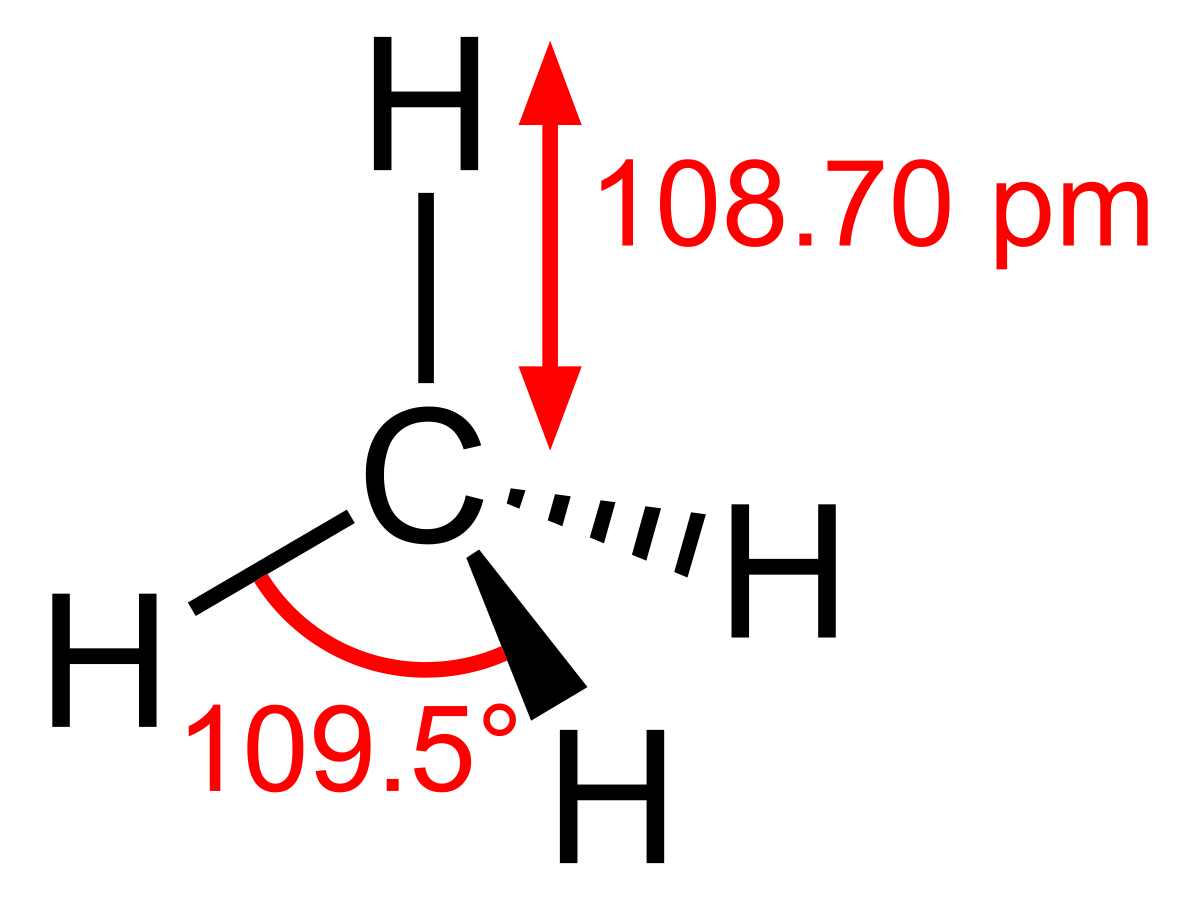
\includegraphics[width=8.75cm]{gambar/metana.png}
		\captionof{figure}{\textit{Senyawa Metana} \cite{Ben2016}}
	\end{center}

	Senyawa organik memiliki pola ikatan tunggal dan rangkap (rangkap dua dan tiga) karena karbon memiliki 4 elektron valensi yang menyebabkan karbon dapat berikatan dengan 4 buah unsur yang berbeda \cite{Clayden2012}. Kimia organik sangatlah berguna untuk produk komersial dan juga produk sains. Seperti contohnya untuk kosmetik, pelumas, bahan petrokimia dan lainnya. Salah satu senyawa kimia organik yang saat ini sedang diteliti yaitu senyawa Graphene / Graphene Oxide.
	
	\section{Graphene Oxide}
	Graphene merupakan senyawa yang terdiri dari miliaran atom karbon (C) yang terbentuk seperti kisi heksagonal (atau sering disebut dengan sarang lebah) dan merupakan struktur fundamental untuk setiap bentuk karbon saat ini \cite{Clemons2010}. Senyawa graphene memiliki karakteristik tebal yang sangat tipis, fleksibel, kuat dan transparan \cite{Ni2015}. Graphene lebih keras daripada Intan, namun lebih elastis daripada karet, lebih kuat daripada Baja dan lebih ringan daripada aluminium \cite{Berger2019}. Graphene merupakan turunan dari karbon yang dijadikan lembaran dan berasal dari graphite.
	
	\begin{center}
		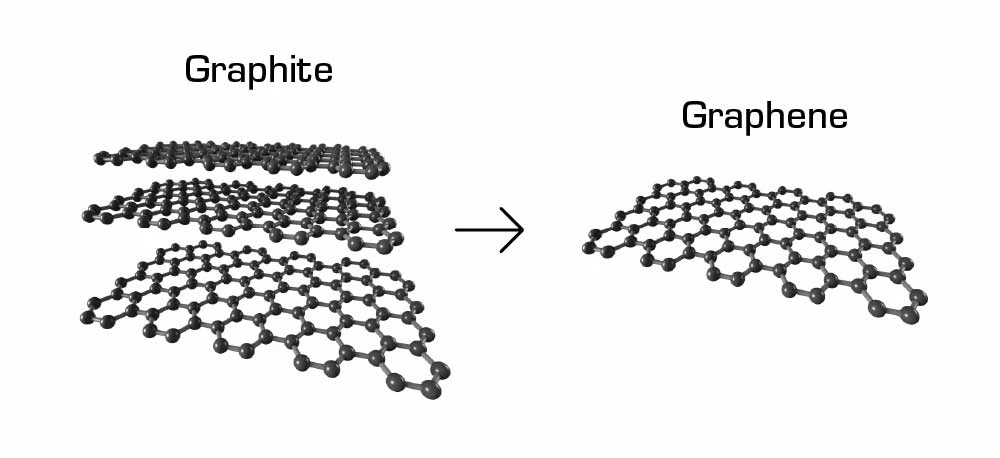
\includegraphics[width=8.75cm]{gambar/grafit.png}
		\captionof{figure}{\textit{Struktur Graphene dan Graphite} \cite{Verjari}}
	\end{center}
	
	Graphene hanya terdiri dari atom C yang jarak antar atom C sebesar ± 0.142 nm \cite{Zhen2017} dan jarak interplanar nya 0.335 nm. Graphene memiliki mobilitas elektron lebih dari
 	15000 $ cm^2 V^{-1} s^{-1} $. Dari sini bisa disimpulkan bahwa Graphene memiliki sifat kimia dan fisiknya yang sangat baik. Lalu karena Graphene adalah dasar dari alotrop grafit, lalu dapat dibentuk menjadi fullerene 0D, digulung menjadi tabung nano (nanotube) 1D, dan ditumpuk menjadi grafit 3D, inilah sebabnya Graphene disebut sebagai induk dari grafit \cite{Chakraborty2018}.
		
	\begin{center}
	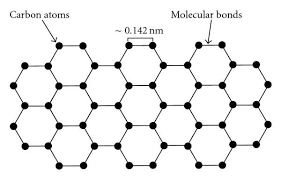
\includegraphics[width=8.75cm]{gambar/grafen.png}
	\captionof{figure}{\textit{Struktur Senyawa Graphene} \cite{Clemons2010}}
	\end{center}
	
	Aplikasi dari Graphene bisa digunakan menjadi resonator, saklar, katup, konduktor dan beberapa aplikasi lainnya \cite{Clemons2010}.
	
	Karena graphene mahal dan relatif sulit untuk dibuat, maka dilakukanlah cara lain yang lebih mudah dan murah untuk membuat senyawa yang seperti graphene. Maka dibuatlah turunannya dengan \textit{dopping} oksida didalamnya yaitu \textit{Graphene Oxide} \cite{MetalgrassLTD2019}. Graphene Oxide dapat dihasilkan dari proses oksidasi Graphite dan jika ingin menghasilkan Graphene murni, maka diperlukan proses reduksi untuk memutus ikatan oksida yang terdapat pada Graphene Oxide. Graphene Oxide memiliki kelebihan yaitu memiliki siklus stabilitas yang lebih baik dibandingkan dengan Graphene, lalu performa yang baik dan yang terpenting mudah diproduksi \cite{Korkmaz2020}. Akibat dari adanya ikatan oksida, maka kapasitansi yang dimiliki oleh Graphene Oxide sangatlah tinggi dan menjadikan Graphene Oxide sebagai bahan yang baik yang digunakan untuk superkapasitor.
	
	\begin{center}
		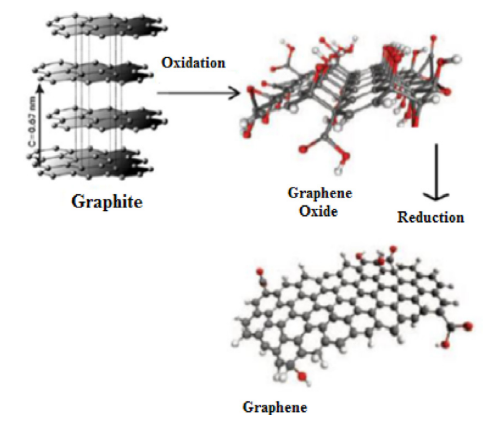
\includegraphics[width=8.75cm]{gambar/oksgraf.png}
		\captionof{figure}{\textit{Pembuatan Graphene dan Graphene Oxide dari Graphite} \cite{Korkmaz2020}}
	\end{center}
	
	Karakteristik dari Graphene bisa kita lihat, salah satunya mengenai energi yang dimiliki oleh orbital molekul Graphene. Untuk melihat energinya, kita dapat menggunakan suatu teori yang dikemukakan oleh Enrich Hückel yang bernama Teori Hückel. 
	
	\section{Teori Hückel}
	Teori Hückel sangat erat kaitannya dengan teori orbital molekul. Orbital molekul merupakan suatu penggambaran daerah yang dapat ditempati oleh suatu elektron dalam suatu molekul. Orbital molekul menggunakan pendekatan Schrödinger untuk elektron dalam medan listrik di inti atom suatu molekul. Dengan menggunakan orbital molekul kita bisa melihat konfigurasi elektron molekul. Karena orbital molekul merupakan fermion, maka ia akan memenuhi prinsip Pauli \cite{Coton1990}. Orbital dari suatu molekul memiliki level energinya masing-masing. Ikatan antar unsur dalam suatu molekul disebut ikatan-{$\sigma$}. Misalkan, senyawa {$C_2H_4$} (etilen), memiliki ikatan C=C dengan ikatan ganda, dan C-H dengan ikatan tunggal. Ikatan C=C dan C-H disebut ikatan-{$\sigma$}, dan karena hibridisasi dari etana memiliki elektron di {$2p_x$} dan {$2p_y$}, maka orbital di {$2p_z$} akan membentuk ikatan-{$\pi$}. Karena jarak antara ikatan-{$\pi$} dan ikatan-{$\sigma$} cukup jauh, menyebabkan interaksi antar ikatan {$\pi$} lebih besar daripada besar interaksi ikatan {$\sigma$} dan {$\pi$}. Maka kita bisa mengabaikan interaksi antara ikatan {$\sigma$} dan {$\pi$} \cite{Siregar2014}\\.
	
	\begin{center}
		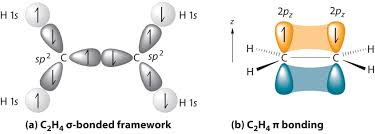
\includegraphics[width=10cm]{gambar/etilen.jpeg}
		\captionof{figure}{\textit{Orbital Molekul Etilen ({$C_2H_4$})} \cite{Anil}}
	\end{center}
	
	Dari sini, Hückel mengembangkan suatu teori dimana orbital molekul yang digunakan dapat dihitung energinya menggunakan teori elektron-{$\pi$}. Maka lahirlah Teori Orbital Molekul Hückel (Teori OMH) atau sering disebut dengan Teori Hückel. Dengan menggunakan teori Hückel, kita bisa melihat energi yang dihasilkan dari ikatan-{$\pi$} suatu molekul. Ia mengungkapkan bahwa orbital molekul yang dilambangkan oleh
	{$\psi$} adalah kombinasi linier dari orbital-orbital {$2p_z$} dari semua atom karbon dalam suatu molekul \cite{Rustaman2008}. Kombinasi linier orbital molekul sering disebut sebagai LCAO (\textit{Linear Combination of Atomic Orbital}) \cite{Maczynski1991}. LCAO {$2p_z$} ini dapat ditulis secara matematis dengan:
	\begin{equation}
	{\psi} = \sum\limits_{i} c_i{\phi}_i
	\end{equation}
	dengan {$\phi_i$} adalah orbital {$2p_z$} dalam atom karbon ke-i. Jika $\hat{H}$ dianggap sebagai Hamiltonian efektif elektron-tunggal dalam molekul, maka berlaku:
	\begin{equation}
	\hat{H}\psi = \epsilon\psi
	\end{equation}
	Persamaan (2.2) memenuhi persamaan sekuler:
	\begin{equation}
	\sum\limits_{j} {H_{ij}}-{\epsilon}{S_{ij}}c_j=0
	\end{equation}
	dengan
	\begin{equation}
	H_{ij} = \int {\phi_i}{\hat{H}}{\phi_j} \,dv
	\end{equation}
	\begin{equation}
	S_{ij} = \int {\phi_i}{\phi_j} \,dv
	\end{equation}
	Integral yang ada di persamaan (2.4) bisa didefinisikan sebagai data empiris. Contohnya adalah {$H_{ii}$} adalah potensial ionisasi elektron-{$\pi$} di karbon ke-i dan {$H_{i,i{\pm}1}$} dalah energi yang dibutuhkan untuk elektron-{$\pi$} melompat ke atom terdekatnya. Karena {$S_{ii}=1$} dan {$S_{ij}$} jauh lebih kecil daripada 1 maka dapat diabaikan. Maka,
	\begin{equation}
	\begin{split}
	\alpha ; i = j
	\\
	H_{ij} = \beta ; j = i{\pm}1
	\\
	0 ; lainnya
	\end{split}
	\end{equation}
	Singkatnya, persamaan diatas dapat menjadi sebuah persamaan matriks yang ditulis dengan,
	\begin{equation}
	\begin{bmatrix}
	{H_{11}-ES_{11}} & {H_{12}-ES_{12}} & ... &{H_{1j}-ES_{1j}}\\
	{H_{21}-ES_{21}} & {H_{22}-ES_{22}} & ... &{H_{2j}-ES_{2j}}\\
	... & ... & ... & ... \\
	{H_{i1}-ES_{i1}} & {H_{i2}-ES_{i2}} & ... &{H_{ij}-ES_{ij}}
	\end{bmatrix}
	\begin{bmatrix}c_1 \\ c_2 \\ ... \\ c_j \end{bmatrix} = 0
	\end{equation}
	Karena {$H_{ii} = \alpha$}, {$H_{ij} = \beta$}, dan {$S_{ij} = \delta_{ij} = 1$} jika {$i=j$} dan akan bernilai 0 jika {$i!=j$}. Maka matriks Hamiltoniannya menjadi,
	\begin{equation}
	\begin{bmatrix}
	\alpha - E & \beta & 0 &\beta \\
	\beta & \alpha - E & \beta & 0\\
	... & ... & ... & ... \\
	\beta & 0 & \beta & \alpha - E
	\end{bmatrix}
	\begin{bmatrix}c_1 \\ c_2 \\ ... \\ c_j \end{bmatrix} = 0
	\end{equation}
	Misalkan pada \textit{Ethylene} memiliki 2 atom C yang menyebabkan matriks Hamiltoniannya menjadi ukuran berukuran 2x2.
	\begin{equation}
	\begin{bmatrix}
	\alpha - E & \beta \\
	\beta & \alpha - E
	\end{bmatrix}
	\begin{bmatrix}c_1 \\ c_2 \end{bmatrix} = 0
	\end{equation}
	Energi orbital molekul dalam teori OMH didefinisikan dalam dua bentuk, yaitu energi dari sebuah elektron dalam orbital 2p yang disebut dengan {$\alpha$} dan energi interaksi antara dua orbital 2p yang disebut dengan {$\beta$} \cite{Anil}\cite{Rustaman2008}.
	
	Dalam kasus ini, {$\hat{H}$} merupakan suatu matriks Hamiltonian yang menggambarkan keadaan orbital dari suatu molekul. Banyaknya atom karbon akan mempengaruhi besar matriks Hamiltonian yang didapat. Seperti misalkan benzene ({$C_6H_6$}) yang memiliki 6 atom karbon, maka matriks yang dihasilkannya berukuran 6x6.
	Jika dikaitkan dengan graphene yang memiliki jumlah atom C yang sangat banyak, maka matriks Hamiltonian yang dihasilkannya pun ukurannya akan sangat besar. Operasi yang akan digunakan yaitu operasi eigen. Hasil dari metode ini adalah energi orbital dari molekul uji yang digunakan. Aplikasi dari metode Hückel ini yaitu bisa menghitung celah pita \cite{Imamura2018}, rapat elektron dan konduktivitas bahan \cite{Siregar2014}.  
	
	Dari penjelasan sebelumnya, permasalahan yang dihadapi yaitu ukuran matriks Hamiltonian yang sangat besar dan ini berefek pada laju komputasi yang akan kita lakukan. Hal tersebut bisa membuat laju komputasi menurun drastis karena proses komputasi yang sangat banyak dan tidak bisa dilakukan secara paralel. Untuk menjawab permaslahan tersebut, maka kita akan menggunakan operasi Block Matrix sebagai paralelisasi operasi matriks agar dapat dikerjakan dengan worker yang berbeda dan membantu dalam komputasi. 
	
	\section{\textit{Block Matrix}}

	\textit{Block Matrix} merupakan salah satu operasi yang paling penting untuk meningkatkan kinerja komputasi. Dengan menggunakan Block Matrix maka operasi dapat diparalelisasi \cite{Davis2004}. Block Matrix adalah operasi matriks dimana suatu matriks berdimensi besar akan dibagi menjadi beberapa sub matriks kecil \cite{Ford2003}.
	
	\begin{center}
		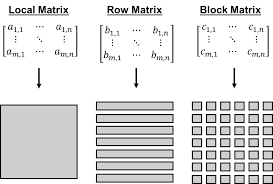
\includegraphics[width=9.1cm]{gambar/blockmat.png}
		\captionof{figure}{\textit{Perbandingan Local Matrix, Row Matrix dan Block Matrix} \cite{Pisciuneri2016}}
	\end{center}
	
	Terlihat dari gambar bahwa Block Matrix akan membagi matriks yang awalnya berukuran sangat besar (yaitu Local Matrix), menjadi beberapa sub matriks kecil. Misalkan kita memiliki matriks A dengan ukuran 4x4,
	\begin{equation}
	A = 
	\begin{bmatrix}
	a_{11} & a_{12} & a_{13} & a_{14} \\
	a_{21} & a_{22} & a_{23} & a_{24} \\
	a_{31} & a_{32} & a_{33} & a_{34} \\
	a_{41} & a_{42} & a_{43} & a_{44}
	\end{bmatrix}
	\end{equation}
	dengan menggunakan Block Matrix, maka matriks A dapat kita bagi menjadi 4 sub matriks yaitu {$A_{11}, A_{12}, A_{21}, A_{22}$}.
	\begin{equation}
	A = 
	\begin{bmatrix}
	A_{11} & A_{12} \\
	A_{21} & A_{22}
	\end{bmatrix}
	\end{equation}
	jika ditulis per submatriksnya menjadi,
	\begin{equation}
	A_{11} = 
	\begin{bmatrix}
	a_{11} & a_{12} \\
	a_{21} & a_{22}
	\end{bmatrix}
	\end{equation}
	\begin{equation}
	A_{12} = 
	\begin{bmatrix}
	a_{13} & a_{14} \\
	a_{23} & a_{24}
	\end{bmatrix}
	\end{equation}
	\begin{equation}
	A_{21} = 
	\begin{bmatrix}
	a_{31} & a_{32} \\
	a_{41} & a_{42}
	\end{bmatrix}
	\end{equation}
	\begin{equation}
	A_{22} = 
	\begin{bmatrix}
	a_{33} & a_{34} \\
	a_{43} & a_{44}
	\end{bmatrix}
	\end{equation}
	Karena elemen matriks yang didapatkan dari Graphene sangat banyak, dan diperlukan adanya sistem komputasi yang bisa memproses banyak data dengan kecepatan yang sangat tinggi. Maka kita akan menggunakan suatu metode menggunakan Big Data.
	
	\section{\textit{Big Data}}
	
	\begin{center}
		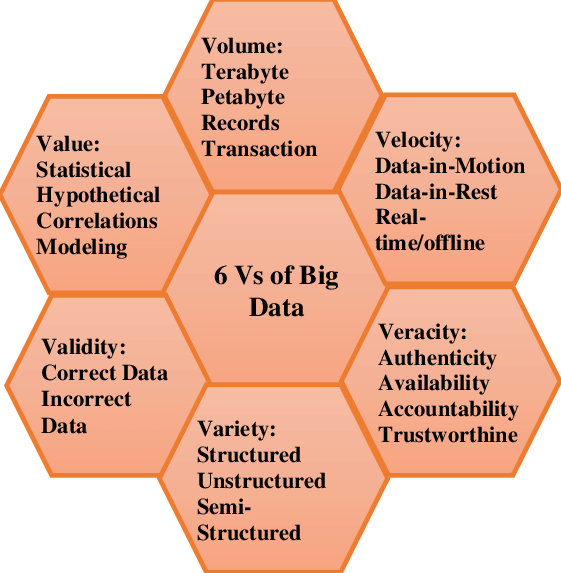
\includegraphics[width=7cm]{gambar/bigdat.png}
		\captionof{figure}{\textit{Big Data dan Karakteristiknya} \cite{Saqlain2017}}
	\end{center}

	\textit{Big Data} adalah salah satu metode cara memproses berbagai jenis data. Data dibagi menjadi dua tipe, yaitu Data Terstruktur (data numerik), dan Data Tidak Terstruktur (teks, suara, gambar, dll) \cite{Shakhovska2019}. Secara makna, Big Data merupakan suatu data yang ukurannya sangat besar, bentuk yang tidak teratur, dengan komunikasi data kecepatan tinggi. Big Data memiliki 6 karakteristik yang disebut sebagai “\textit{6V’s of Big Data}” yang tertera pada Tabel 2.1.
	
	\begin{table}[h]
		\centering
		\caption{Karakteristik Big Data \cite{Moura2015}\cite{Schaafsma2020}}
		\label{tab:my_label}
		\begin{tabular}{|p{0.2\linewidth} | p{0.7\linewidth}|} 
			\hline
			Volume\centering & Volume adalah salah satu hal yang menjadi feature dari Big Data. Berkaitan dengan hubungan antara ukuran dan kapasitas pemrosesan. \\ \hline
			Velocity\centering & Kecepatan pemrosesan Big Data sangatlah cepat, ini dikarenakan dari data yang dimilikinya sangat besar dan akan semakin membesar seiring banyaknya data yang masuk. Kecepatan yang dimiliki sangat cepat karena memanfaatkan data geolokasi, tren dan informasi input data. \\ \hline
			Value\centering & Value menjelaskan bahwa nilai yang akan diperoleh dari suatu data dan lebih bernilai dari stored data \\ \hline
			Variability\centering & Variability mengungkap tentang variable-variabel yang mempengaruhi proses komunikasi data dan pemrosesannya beserta kemungkinan terbaiknya. \\ \hline
			Veracity\centering & Veracity menunjukkan kualitas dan asal data, dan sebagai penyeleksian kebenaran dan keaslian data. \\ \hline
			Variety\centering & Variety menggambarkan bahwa didalam Big Data terdapat banyak variasi atau macam data yang akan diproses dan dianalisis. Bise berupa data numerik, audio video, bahkan teks. \\ \hline
		\end{tabular}
	\end{table}

	Big Data biasa disebut sebagai Not-Only Structured Query Language (NoSQL), hal ini berbeda dengan Relational Database Management System (RDBMS) atau basis data tradisional mulai dari variasi data untuk NoSQL bisa mencakup data semi terstruktur dan data tidak terstruktur, kecepatan baca-tulis (Read-Write) data dari Big Data yang sangat cepat (bergantung pada jumlah node) dan scalable \cite{Fadillah2020}. Beberapa kelebihan dan kekurangan menggunakan Big Data terdapat pada Tabel 2.2.
	
	\begin{table}[h]
		\centering
		\caption{Kelebihan dan Kekurangan Big Data \cite{Harvey2018}}
		\begin{tabular*}{\linewidth}{|p{0.44\linewidth}|p{0.5\linewidth}|}
			\hline
			Kelebihan & Kekurangan \\ \hline
			Pengambilan keputusan yang lebih baik & Kebutuhan akan \textit{talent} yang profesional di bidangnya \\ \hline
			Peningkatan produktivitas & Kualitas data \\ \hline
			Mengurangi biaya & Perlunya perubahan budaya untuk menggunakan Big Data \\ \hline
			Peningkatan layanan pelanggan & Peraturan yang mengatur tentang privasi data \\ \hline
			Deteksi penipuan & Resiko keamanan \\ \hline
			Peningkatan pendapatan & Perubahan yang cepat \\ \hline
			Peningkatan agility & Kebutuhan perangkat keras pendukung \\ \hline
			Inovasi yang lebih besar & Kecepatan lebih cepat dalam pemrosesannya  \\ \hline
			Kecepatan lebih cepat dalam pemrosesannya & Biaya \\ \hline
		\end{tabular*}
	\end{table}
	Terdapat beberapa \textit{platform} yang sering digunakan dalam pengolahan Big Data, dan beberapa dan yang akan digunakannya adalah Apache Kafka dan Apache Spark. 
	
	\subsection{\textit{Apache Spark}}
	\begin{center}
		
\includegraphics[width=8.7cm]{gambar/spark.png}
		\captionof{figure}{\textit{Apache Spark} \cite{Apache2018}}
	\end{center}
	Apache Spark merupakan sebuah aplikasi mesin analitik yang terpadu untuk pemrosesan data berskala besar \cite{Apache2018}. Apache Spark banyak digunakan di berbagai industri, seperti Netflix, Yahoo, dan eBay. Kelebihan dari Spark adalah:
	\begin{enumerate}
		\item Kecepatan\\
		Spark memiliki kecepatan 100x lebih cepat daripada Hadoop. Ini karena Spark menggunakan komputasi dan beberapa pengoptimalan lainnya. 
		\item Kemudahan dalam penggunaan\\
		Spark memiliki antarmuka yang mudah digunakan untuk memproses Big Data.
		\item Aplikasi terpadu\\
		Spark memiliki dukungan dan library yang sangat banyak, termasuk SQL, streaming data, machine learning, dan pemrosesan grafik. Salah satunya, spark dapat dioperasikan menggunakan library dari python yang disebut sebagai PySpark. Library inilah yang akan digunakan untuk melakukan komputasi pada tugas ini \cite{Databricks}. 
	\end{enumerate}

\chapter*{BAB III \\ METODE PENELITIAN}
\addcontentsline{toc}{chapter}{BAB III METODE PENELITIAN}
\setcounter{chapter}{3}
\setcounter{section}{0}
\setcounter{figure}{0}
\setcounter{equation}{0}
\thispagestyle{myplain}

Penelitian Kalkulasi Nilai Eigen berbasis Matriks Hamiltonian menggunakan Teknik \textit{Block Matrix} : Studi Kasus Pada \textit{Graphene} / \textit{Graphene Oxide} dilakukan dengan 3 tahapan, yaitu perancangan algoritma penelitian, perancangan kode komputasi dan simulasi data. Perancangan algoritma penelitian akan membuat cara kerja aplikasi yang akan dibuat dimulai dari \textit{Start} hingga komputasi berakhir. Dalam perancangan kode komputasi akan dibuat kode berbahasa \textit{Python} yang akan dieksekusi oleh PySpark. Tahap terakhir adalah simulasi data. Simulasi data akan mensimulasikan kode yang sudah dibuat menggnakan perangkat komputer dengan spesifikasi yang ditentukan. Dari hasil simulasi data ini akan dilihat validitas dan performa komputasi yang dihasilkan.

	\section{Perancangan Algoritma Penelitian}
		Langkah-langkah penelitian dapat dilihat pada diagram alir penelitian pada Gambar 3.1
	\begin{center}
		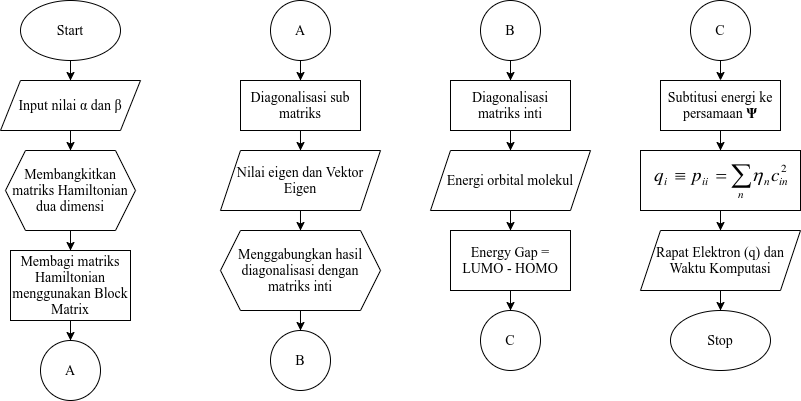
\includegraphics[width=12cm]{gambar/diagram_alir.png}
		\captionof{figure}{Diagram Alir Penelitian}
	\end{center}
	 Dalam penelitian ini, akan dilakukan dengan beberapa tahap, yaitu pendefinisian, pemecahan matriks utama menjadi sub matriks kecil, diagonalisasi matriks, dan subtitusi untuk dapat keluaran besar energi orbital molekul dari graphene dan laju konvergensi yang didapatkannya. Diawali dengan penginputan besar {$\alpha$} dan {$\beta$} dari Graphene Compound lalu akan dibangkitkan matriks Hamiltoniannya. Lalu, matriks Hamiltoniannya akan dibagi menjadi 4 sub matriks untuk dapat dikerjakan secara paralel. Tiap sub matriks tersebut akan didiagonalisasi untuk mendapatkan nilai eigennya. Hasil dari diagonalisasi sub matriks akan digabung menjadi matriks utuh seperti matriks utama dan didiagonaliasi kembali. Keluaran dari sini adalah besar konstanta yang didapatkan. Besar konstanta kemudian disubstitusi ke persamaan awal untuk mendapatkan nilai energi orbital molekul. Laju konvergensinya akan diplot untuk melihat besar error yang didapat tiap iterasinya.
	\section{Alat yang Digunakan}
			\subsection{Perangkat Lunak}
			\begin{enumerate}
				\vspace{-0.2cm} \item \textit{Apache Spark} versi 3.0.1
				\vspace{-0.8cm} \item \textit{Visual Studio Code} versi 1.52.1
				\vspace{-0.8cm} \item \textit{Gnuplot} versi 5.2 \textit{patchlevel} 8
			\end{enumerate}
		
			\subsection{Perangkat Keras}
			\begin{enumerate}
				\vspace{-0.2cm}\item Prosessor AMD Ryzen 5 2500u 8 \textit{core} 16 \textit{thread}
				\vspace{-0.8cm} \item RAM 2x8 GB 2666 MHz DDR 4
				\vspace{-0.8cm} \item GPU Radeon Vega 8 Graphics
				\vspace{-0.8cm} \item Antarmuka Ubuntu 20.04.1
			\end{enumerate}
	\section{Perancangan Kode Komputasi}
	Pada perancangan kode komputasi ini akan membuat kode dalam bahasa \textit{Python} yang akan dikonversi menjadi kode yang dapat dieksekusi di \textit{PySpark}. Matriks Hamiltonian yang dimiliki oleh Graphene Oxide bersifat matriks dua dimensi. Lalu dalam penentuan ikatan nya akan dilakukan menggunakan penentuan posisi atom acak dua dimensi. Penentuan posisi {$\vec{A}$} yaitu dengan
	\begin{equation}
	\vec{A} = A_x + A_y
	\end{equation}
	\begin{equation}
	A_x = rand * L_x
	A_y = rand * L_y
	\end{equation}
	dengan rand = angka acak, dan
	{$L_x$} = {$L_y$} = panjang horizontal dan vertikal.\\
	Untuk menentukan indeks cell dari matriks dapat menggunakan rumus:
	\begin{equation}
	index = A_y * L_x + A_x
	\end{equation}
	Maka, dari indeks yang dihasilkan akan menjadi matriks seperti berikut
	\begin{equation}
	\begin{bmatrix}
	index_{11} & index_{12} & index_{13} \\
	index_{21} & index_{22} & index_{23} \\
	index_{31} & index_{32} & index_{33}
	\end{bmatrix}
	\end{equation}
	atau jika dijadikan angka indeks,
	\begin{equation}
	\begin{bmatrix}
	9 & 8 & 7 \\
	6 & 5 & 4 \\
	3 & 2 & 1
	\end{bmatrix}
	\end{equation}
	
	Angka indeks inilah yang akan digunakan dalam pembuatan fungsi matriks Hamiltonian.\\
	
	Kemud
	
	
\chapter*{BAB IV \\ HASIL DAN PEMBAHASAN}
\addcontentsline{toc}{chapter}{BAB IV HASIL DAN PEMBAHASAN}
\setcounter{chapter}{4}
\setcounter{section}{0}
\setcounter{figure}{0}
\setcounter{equation}{0}
\thispagestyle{myplain}

\section{Perancangan Algoritma Penelitian}

\section{Perancangan Kode Komputasi}


\chapter*{BAB V \\ KESIMPULAN DAN SARAN}
\addcontentsline{toc}{chapter}{BAB V KESIMPULAN DAN SARAN}
\setcounter{chapter}{5}
\setcounter{section}{0}
\setcounter{figure}{0}
\thispagestyle{myplain}
	
\addcontentsline{toc}{chapter}{DAFTAR PUSTAKA}
\printbibliography[title = {DAFTAR PUSTAKA}]

\end{document}
